\subsection{Fluxions Identification} \label{chapter5:flx:compiler}

The source languages we focus on should offer higher-order functions and be implemented as an event-loop with a global memory.
Javascript is such a language and is often implemented on top of an event-loop, like in \textit{Node.js}.
We developed a compiler that transforms a \textit{Node.js} application into a fluxional application compliant with the execution model described in section \ref{section:model}.
Our compiler uses the \textit{estools}\ftnt{https://github.com/estools} suite to parse, manipulate and generate source code from Abstract Syntax Tree (AST).
And it is tailored for -- but not limited to -- web applications using \textit{Express}\ftnt{http://expressjs.com/}, the most used \textit{Node.js} web framework.

\begin{figure}
  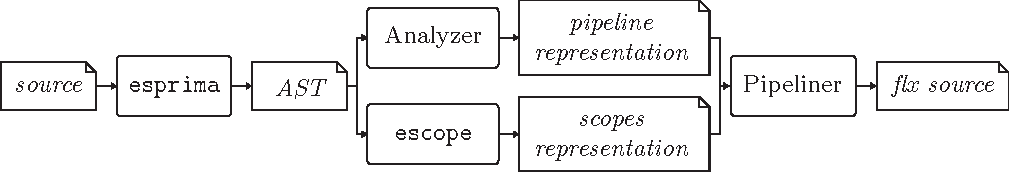
\includegraphics[width=\linewidth]{../resources/compiler-stream.pdf}
  \caption{Compilation chain}
  \label{fig:compilation}
\end{figure}

The chain of compilation is described in figure \ref{fig:compilation}.
The compiler extracts an AST from the source with \texttt{esprima}.
From this AST, the \textit{Analyzer} step identifies the limits of the different application parts and how they relate to form a pipeline.
This first step outputs a pipeline representation of the application.
Section \ref{chapter5:flx-compiler:analyzer} explains this first compilation step.
In the pipeline representation, the stages are not yet independent and encapsulated into fluxions.
From the AST, \texttt{escope} produces a representation of the memory scopes.
The \textit{Pipeliner} step analyzes the pipeline representation and the scopes representation to distribute the shared memory into independent groups of fluxions.
Section \ref{chapter5:flx-compiler:pipeliner} explains this second compilation step.

% \subsubsection{Analyzer step} \label{chapter5:flx-compiler:analyzer}

The limit between two application parts is defined by a rupture point.
The analyzer identifies these rupture points, and outputs a representation of the application in a pipeline form.
Application parts are the stages, and rupture points are the message streams of this pipeline.

\subsubsection{Rupture points} \label{chapter5:flx-compiler:analyzer:rupture}

A rupture point is a call of a loosely coupled function.
It is an asynchronous call without subsequent synchronization with the caller.
In \textit{Node.js}, I/O operations are asynchronous functions and indicate rupture points between two application parts.
Figure \ref{fig:basicrp} shows a code example of a rupture point with the illustration of the execution of the two application parts isolated into fluxions.
The two application parts are the caller of the asynchronous function call on one hand, and the callback provided to the asynchronous function call on the other hand.

\begin{figure}[h!]
  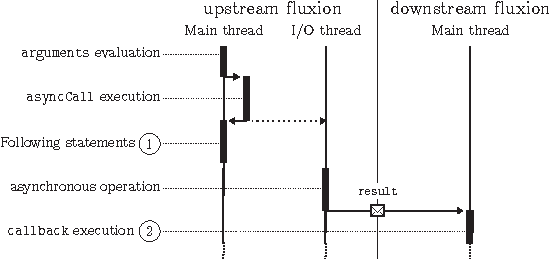
\includegraphics[width=\linewidth]{../resources/basicrp.pdf}
  \begin{code}
asyncCall(arguments, function callback(result){ //@\circled{2}@ });
// Following statements //@\circled{1}@
  \end{code}
  \caption{Rupture point interface}
  \label{fig:basicrp}
\end{figure}

A callback is a function passed as a parameter to a function call.
It is invoked by the callee to continue the execution with data not available in the caller context.
There are three kinds of callbacks, but only two are asynchronous: listeners and continuations.
The two corresponding types of rupture points are \textit{start} and \textit{post}.

\textbf{Start rupture points} (listeners) are on the border between the application and the outside, continuously receiving incoming user requests.
An example of a start rupture point is in listing \ref{lst:source}, between the call to \texttt{app.get()}, and its listener \texttt{handler}.
These rupture points indicate the input of a data stream in the program, and the beginning of a chain of fluxions to process this stream.

\textbf{Post rupture points} (continuations) represent a continuity in the execution flow after an asynchronous operation yielding a unique result, such as reading a file, or a database.
An example of a post rupture points is in listing \ref{lst:source}, between the call to \texttt{fs.readFile()}, and its continuation \texttt{reply}.

\subsubsection{Detection}

The compiler uses a list of common asynchronous callees, like the \texttt{express} and file system methods.
This list can be augmented to match asynchronous callees individually for any application.
To identify the callee, the analyzer walks the AST to find a call expression matching this list.

After the identification of the callee, the callback needs to be identified as well, to be encapsulated in the downstream fluxion.
For each asynchronous call detected, the compiler tests if one of the arguments is of type \texttt{function}.
Some callback functions are declared \textit{in situ}, and are trivially detected.
For variable identifiers, and other expressions, the analyzer tries to detect their type.
The analyzer walks back the AST to track their assignations and modifications, so as to determine their last value.





% \comment{TODO insert this}
% We developed the compiler core in node.js Javascript.
% There already exist sets of tools for manipulating code in Javascript.
% We used the Esprima suite of tools.